

\documentclass{acm_proc_article-sp}
\usepackage{float}% If comment this, figure moves to Page 2
\usepackage{epstopdf}
\usepackage{pstricks}
\usepackage{graphicx}
\usepackage{placeins} 
\begin{document}

%\title{A Sample {\ttlit ACM} SIG Proceedings Paper in LaTeX
%Format\titlenote{(Does NOT produce the permission block, copyright information nor page numbering). For %use with ACM\_PROC\_ARTICLE-SP.CLS. Supported by ACM.}}
\title{GPSInsights: Towards an efficient framework for storing and mining massive real-time vehicle location data}

%\subtitle{[Extended Abstract]

%\titlenote{A full version of this paper is available as
%\textit{Author's Guide to Preparing ACM SIG Proceedings Using
%\LaTeX$2_\epsilon$\ and BibTeX} at
%\texttt{www.acm.org/eaddress.htm}}
%}
%
% You need the command \numberofauthors to handle the 'placement
% and alignment' of the authors beneath the title.
%
% For aesthetic reasons, we recommend 'three authors at a time'
% i.e. three 'name/affiliation blocks' be placed beneath the title.
%
% NOTE: You are NOT restricted in how many 'rows' of
% "name/affiliations" may appear. We just ask that you restrict
% the number of 'columns' to three.
%
% Because of the available 'opening page real-estate'
% we ask you to refrain from putting more than six authors
% (two rows with three columns) beneath the article title.
% More than six makes the first-page appear very cluttered indeed.
%
% Use the \alignauthor commands to handle the names
% and affiliations for an 'aesthetic maximum' of six authors.
% Add names, affiliations, addresses for
% the seventh etc. author(s) as the argument for the
% \additionalauthors command.
% These 'additional authors' will be output/set for you
% without further effort on your part as the last section in
% the body of your article BEFORE References or any Appendices.

\numberofauthors{3} %  in this sample file, there are a *total*
% of EIGHT authors. SIX appear on the 'first-page' (for formatting
% reasons) and the remaining two appear in the \additionalauthors section.
%
\author{
% You can go ahead and credit any number of authors here,
% e.g. one 'row of three' or two rows (consisting of one row of three
% and a second row of one, two or three).
%
% The command \alignauthor (no curly braces needed) should
% precede each author name, affiliation/snail-mail address and
% e-mail address. Additionally, tag each line of
% affiliation/address with \affaddr, and tag the
% e-mail address with \email.
%
% 1st. author
\alignauthor
Hoang L. Truong\\
       \affaddr{Hanoi University of Technology}\\
       \email{linhth.k55.hust@gma-il.com}
% 2nd. author
\alignauthor
Duy K. Bui\\
       \affaddr{Hanoi University of Technology}\\
       \email{duykhanh1412@gma-il.com}
% 3rd. author
\alignauthor
Viet T. Trung\\
       \affaddr{Hanoi University of Technology}\\
       \email{trungtv@soict.hu-st.edu.vn}
}
% There's nothing stopping you putting the seventh, eighth, etc.
% author on the opening page (as the 'third row') but we ask,
% for aesthetic reasons that you place these 'additional authors'
% in the \additional authors block, viz.
\additionalauthors{Additional authors: John Smith (The Th{\o}rv{\"a}ld Group,
email: {\texttt{jsmith@affiliation.org}}) and Julius P.~Kumquat
(The Kumquat Consortium, email: {\texttt{jpkumquat@consortium.net}}).}
\date{30 July 1999}
% Just remember to make sure that the TOTAL number of authors
% is the number that will appear on the first page PLUS the
% number that will appear in the \additionalauthors section.

\maketitle
\begin{abstract}
Intelligent Transport System (ITS) has seen growing interest in collecting vehicle location data in order to build up real-time traffic monitoring and analytic systems. However handling these data creates challenges, as they are massive in volume and arriving in near real-time. In this paper, we proposed GPSInsights, a distributed system that is scalable and efficient in processing huge volume of location data stream. GPSInsights is built up on open-source, scalable and distributed components. We demonstrated our system with a scalable map matching implementation and performed experiments with real big datasets. 

% A category with the (minimum) three required fields
\category{H.4}{Information Systems Applications}{Miscellaneous}
%A category including the fourth, optional field follows...
\category{D.2.8}{Software Engineering}{Metrics}[complexity measures, performance measures]

\terms{Bigdata}

\keywords{GPSInsights, spatio-temporal data storage, distributed data processing, map matching}
\end{abstract}

\section{Introduction}


With the widespread adoption of GPS technology, Intelligent Transport System~(ITS) has seen growing interest in collecting location data of transport vehicles. This data collection is done with the purpose of being able to deliver not only real-time traffic monitoring but also useful traffic statistics and predictive information. Lee et al.~\cite{Lee2011} presented a data mining algorithm to discover traffic bottlenecks. Demiryurek et al.~\cite{Demiryurek2010} proposed an online computation for optimal traffic routes based on traffic data. However, none of these approaches discuss how to implement the system at large-scale.


According to Decree No. 91/2009/ND-CP of Ministry of Transport of Vietnam, all Vietnamese-licensed cars in must be equipped with a standardised global positioning system (GPS) (black-box) which reports geo-location, speed and direction every 30 seconds to a centralised data center. With nearly 200.000 cars in circulation in the near future, the data is enormous and has big data characteristics. First, data is generated continuously in big volume (e.g. petabytes (PB)) from hundred thousand of vehicles. Second, in-coming data rate is near real-time, at which the underlying system must deliver. Third, data has big value for the potential insights about the current situation of the traffic infrastructure as well as for the predictions. 


As big data create non-conventional challenges, current ITS management systems storing data in relational database systems (e.g. via PostGIS~\cite{posgis}) will not be able to adapt to the data ingestion rate, nor being able to be processed efficiently. In this work, we describe GPSInsights: a novel scalable system for storing and mining massive real-time vehicle location data. GPSInsights is able to handle increasingly huge volume of data (~PB) while supporting real-time analytics. We demonstrates GPSInsights with a scalable map matching implementation. 

This paper is organised in 7 parts. In Section~2, we discuss an overall architecture of our system framework. In Section~3, we go into the details of the technologies and components of GPSInsights. In Section~4, we establish a simple demonstration map matching algorithm. Section~5 presents experimental results for the algorithm presented in Section~4. Section~6 discusses related works on existed map matching algorithms and on storing spatio-time data. We conclude and discuss future work in Section~7.
	
\section{System design} 

We design GPSInsights with the following components as depicted  in Figure~\ref{architecture}

\begin{figure}[h]
\centering
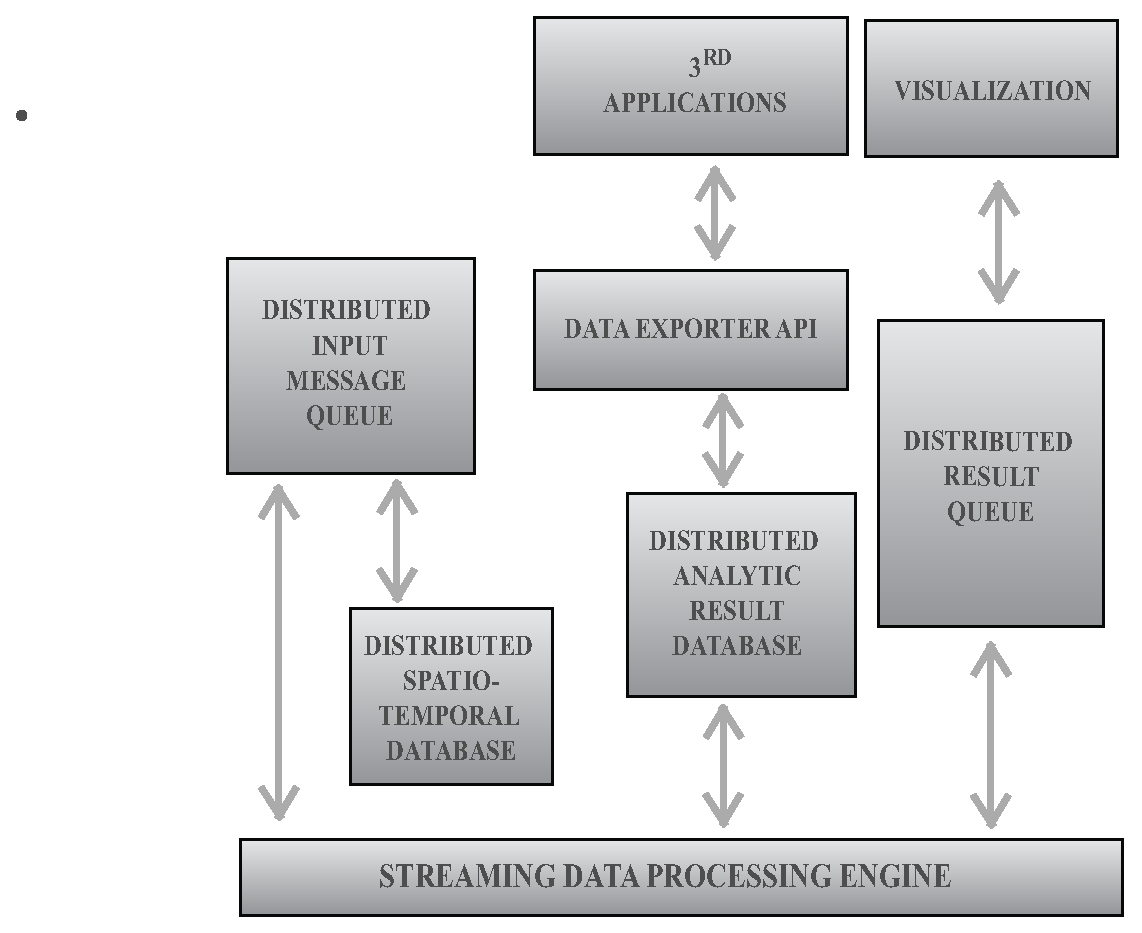
\epsfig{file=architecture.eps, height=175px, width=220px}
\caption{The architecture of the system}
\label{architecture}
\end{figure}

\begin{itemize}
\item 	Distributed input message queue: As the location data arrive from a huge number of source vehicles continuously, this component is responsible for combining the multi-source data, and putting them in their chronological order. It has to store and replicate the large input data dispersedly on a large cluster for high-throughput, and for fault-tolerance. The distributed message queue implements producer-consumer skeleton in which GPS devices installed on transportation vehicles are the producers and the storage engine or the processing engine of GPSInsights become the consumers.

\item  Streaming data processing engine: To allow realtime analytics, GPSInsights powers a streaming data processing engine. This component has to be able to analyse data ``on the fly'', which then outputs analytic reports such as average speed, number of vehicles, and traffic bottleneck prediction. It has to be scaled out on thousand of servers to adapt to the workload.

\item  Distributed result queue: Results from the data processing engine are sent to this component. This acts as the interface to continuous consumer services at application level such as web, mobile apps. 

\item  Distributed spatio-temporal database: As location data consist of geolocation information and timestamp in which the data is recorded, GPSInsights stores data in a distributed spatio-temporal database. This components aims to provide the spatial querying and data manipulation as PostGIS but at large-scale for offline phase. 

\item  Distributed analytic result database. This database is selected to store the analytic results from the data processing engine, acting as the datastore for both display services at the application level and offline processing systems. 

\end{itemize}


\section{Implementation} 

With the system architecture shown in Chapter~2, we build our GPSInsights using open-source components with custom plugins to satisfy our design goals. By leveraging existing components, we can develop GPSInsights quickly and focus on the scalability aspect of the entire system. Thus, a part of our contribution is to design the system overall, to carefully extend the right components, and to run the experiments with real datasets.  

\begin{figure}[h]
\centering
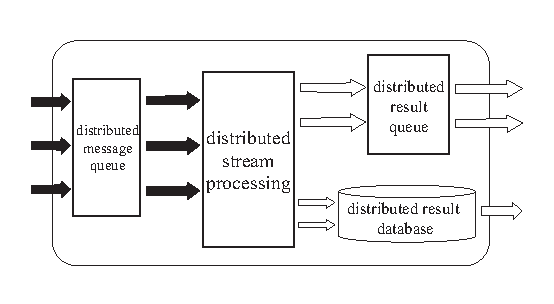
\epsfig{file=architectureOfSystem.eps, height=100px, width=220px}
\caption{The detailed architecture of the system}
\end{figure}

\subsubsection{Apache Kafka.} 

Apache Kafka~\cite{kafkapaper,kafkaweb} is a distributed publish-subscribe messaging service with the purpose of being fast, scalable and durable. Kafka maintains feeds of messages in categories called topics. Each topic is a partitioned log, distributed over multiple cluster server nodes as in Figure~\ref{architecture}. Inside a particular partition, the messages are immutable and ordered, identified by an ``offset''. This design choice allows not only storing the amount of the data larger than the capability of any single node but also parallelizing read and write operations. Technically, the producer that publish messages can distribute messages over multiple partitions of a topic in a round-roubin fashion, or it can distribute according to some semantic partition functions.

Kafka achieve fault-tolerance by replicating partitions across a configurable number of nodes. Each partition has one ``leader'' and several ``follower'' nodes. The ``leader'' node serves all read and write requests for the partition while the followers are mirroring. Once the leader failed, one of the follower will be automatically promoted to be the new leader (using the well-known distributed leader election algorithm). In production, every Kafka node acts as leader for some partitions and follower for others to achieve balancing. 

In GPSInsights, Kafka is used for the distributed input message queue and the result queue. With suitable configuration, Kafka helps GPSInsights agregating in-coming location data and route analytics results to the appropriate layers (E.g. to the storage and to the end-user applications).

\subsubsection{Spark Streaming and Storm.}

Spark Streaming~\cite{learningsparkbook,sparkstreamingweb} and Apache Storm~\cite{stormappliedbook,apachestormweb} are the most popular open-source frameworks for distributed stream processing. In distributed mode, both of them use a master/slave architecture with one central coordinator and many distributed workers. However, there are still the important differences in their architectures as following.

Spark Streaming lays on top of Apache Spark~\cite{Zaharia:2010:SCC:1863103.1863113} for acting on data stream.
 At the core of Spark Streaming is the concept of discretized abstraction (D-streams)~\cite{Zaharia:2013:DSF:2517349.2522737,Zaharia:2012:DSE:2342763.2342773}, that considers in-coming records as a series of deterministic batchs on small time intervals. Each batch is treated as a reslient distributed dataset (RDD) of Spark, and being processed using RDD operations. 

 Spark's RDDs offer fault-tolerance and parallel computation at large-scale though three important design principles. First, RDD is partitioned in chunks, distributed across compute nodes (as in Hadoop Mapreduce paradigm). Second, every computations within RDD are recorded in logs (called lineage). Third, temporary data is kept in memory to speed up computation. If any partition of an RDD is lost due to a node failure, as long as the source the input data which is usually at immutable Hadoop file system HDFS~\cite{shvachko2010hadoop}, then that partition can be re-computed from it using the lineage of operations.

Instead of batching up events that arrive within a short time and then process them as in Spark Streaming, Storm processes incoming events one at a time (so storm's processing latency could be sub-second, while Spark Streaming reaches a latency of several seconds). The work in Storm is delegated to different types of components that are responsible for a specific processing task. The input data stream are received by a specialized component called a ``spout''. Then the spout immediately passes the data to another component called a ``bolt''. In a bolt, the data will be transformed in some way, and the bolt either sends it to some sort of storage or passes it to some other bolt. In general, a Storm cluster can be considered as a network of bolt components in which each one applies some kind of transformation on the data receiving from the spout, the arrangement of spouts and bolts and their connections in the cluster is called a topology. In storm, each individual record has to be tracked when moving through the system. However, Storm only guarantees that each record will be processed at least once.

GPSInsights is implemented to work with both Spark Streaming and Storm as the stream processing engine.

\subsubsection{MongoDb.}


Because of the rapid increase in velocity and volume of the result data, Traditional relational databases are no longer the ``one-size-fits-all'' for every type of data. They do not scale well to large datasets because their scaling model is vertial: more data means bigger server. One way to scale relational databases across multiple server is to do ``database sharding''. However, this mechanism is limited scalability due to the inherent complexity of the relational interface and the ACID (atomicity, consistency, isolation, and durability) guarantees. 

MongoDB~\cite{mongodbweb} is a document store with the posibility to scale horizontally. It is designed for managing semi-structured data organized as a collection of documents. In MongoDB, the structure of the documents is very flexible. There is no pre-defined scheme as the columns, and colume datatypes as in relational databases. MongoDB distributes documents by the document IDs across servers and implements replication for fault-tolerance. When comparing the performance between the two different databases~\cite{10.11648/j.ajsea.20150402.12}, MongoDb saw the much better performance than MySQL - the traditional relational database.

GPSInsights uses MongoDB to store the statistic results from the data processing engine. GPSInsights leverages the ability of MongoDB to write data fast and in a flexible scheme. 

\subsubsection{Geomesa.}
 
Geomesa~\cite{fox2013spatio} is an open-source, distributed, spatio-temporal data-base built on top of a column-family oriented distributed database called Accumulo~\cite{accumuloonline}. Geomesa uses a very flexible strategy to linearize geo-time data. It distributes the data across the nodes in a cluster to leverage parallelism, thus enables efficient storing, querying, and transforming large spatio-temporal data. Geomesa is like PostGIS~\cite{posgis} but at very large-scale and for big data workloads. 

GPSInsights relies on Geomesa for storing raw in-coming location data which will be the input for doing batch processing if necessery. Note that GPSInsights focuses on real-time analytics but it also features long running analytic jobs. Those will be discussed in the future papers. 

\subsubsection{Guarantee realibility}

The primary reason of choosing the distributed message queue as a component of GPSInsights is to minimize the number of data loss when the system fails. In the case of lacking the message queue component, the data processing engine would directly receive the data from the GPS devices. Once a master node of the processing engine dies (the master node of Spark called ``driver program'', one of Storm called ``Spout''), GPSInsights will not receive and handle any data which arrive, thus those transportation data will be totally lost. By contrast, with the message queue, GPSInsight can ensure zero transportation data loss (the message queue is fault-tolerance as Kafka). When recovering, the processing engine will pull the next unprocessed data from the queue to continue handling.

However, GPSInsights have to deal with unrealiability even with the support of message queues. There are two challenges. 

First, how to guarantee that the output data from Spark Streaming were completely sent to MongoDb? Data lost happens when Spark Streaming goes wrong and not pushes all the result data to the result database. MongoDb in this case receives the incomplete set of the data, but Spark Streaming supposes it completed the task with the current batch and then continued handling the next batch.

\begin{figure}[h]
\centering
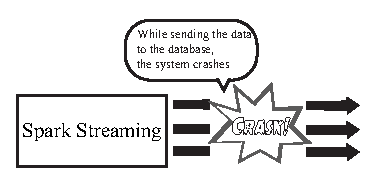
\epsfig{file=sendingcrash.eps, height=100px, width=220px}
\caption{The first problem}
\end{figure} 

Second, some messages might appear repetitively in a batch due to failures that the Spark Streaming Receiver failed to inform Kafka about its current received messages. Therefore, Spark Streaming supposed it received the data, but Kafka supposed that the messages was not sent successfully and would resend repetitively. 
 
\begin{figure}[h]
\centering
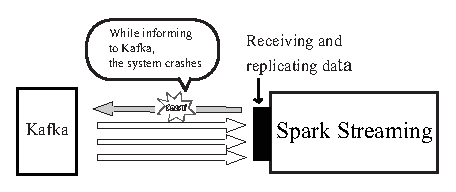
\epsfig{file=receivingcrash.eps, height=100px, width=220px}
\caption{The second problem}
\end{figure} 

The two above problems is caused by the fact that each component of GPSInsights cannot know exactly whether the data are handled fully by the other components. To overcome these, there should be a mechanism to maintain a consistent view of what has been processed successful by the system. Therefore, we have to introduce a transaction guarantee to GPSInsights to ensures that either all output data from Spark Streaming are logged to MongoDB or the arriving data are reprocessed.

To achieve this guarantee, first, we implemented a new Spark Streaming's Receiver by using the Spark Streaming's ``receiverStream'' API and the Kafka's Simple Consumer API ~/cite{kafkasimpleapi}. Instead of handling only the latest data, the new Spark Streaming Receiver can specify the start position of the offset for each partition at the beginning of every batch interval. It can also get the extra information of each record including its offset, id of the partition which it belongs to. Second, we created a MongoDb database with three different collections, namely ``Transactions'', ``Records'', and ``OffsetRanges''. The ``Transaction'' consists of documents having three fields: id, timestamp and status. The status field can accept two value: ``BEGIN'' means the beginning of a transaction and ``FINISH'' expresses the end of the transaction. ``Records'' contains documents which are the information of the analytic results from Spark Streaming and an id of the transaction. ``OffsetRanges'' includes documents which hold the information of an offset range of the records packaged into the current batch, and the id of the transaction.

The detail implementation is described as follows. Before sending to Spark Streaming's Receiver, each record in Kafka will be attached with its offset and partition's id which it belongs to. Using Accumulator API ~\cite{accumulatorapi}, we can find the offset range of each Kafka's partition in the current batch. When finishing handling this batch and before logging the result data to MongoDb, we create a new document with ``Begin'' status in ``Transactions'' collection and get its id. We then create a new document in ``OffsetRanges'' collection with the offset range and the id. Next, we send the result data to ``Records'' collection, attaching the id. Finally, after the last record is written successful in MongoDb, we change the status field of the transaction to ``Finish'', and the current batch is handled successful. During running, if the system fails and then recovers, it will query MongoDb for the last document in ``Transactions'' collection.  If the value of the status field is ``Finish'', it means the process of handling the last batch was succeeded. By contrast, we will use the transaction id to get the relevant document in ``OffsetRanges'' collection, and use the first offset in each ranges (the number of range is equal to the number of partition of the Kafka' topic that we are consuming) to recomputed the data. 

\section{Scalable map matching}

In this section, we demonstrate how GPSInsights handles the map matching job in a scalable way. Map matching job aims at associating location data to the road network on a digital map. This is the first and the required step for many location data mining algorithms. 

\begin{table}[h]
\centering
\begin{tabular}{|c|c|c|c|c|}
\hline
\textbf{time\_stamp} & \textbf{car\_id} & \textbf{lon}   & \textbf{lat} & \textbf{speed} \\ \hline
\end{tabular}
\end{table}
	
\subsection{General strategy} \label{ssec:links}

GPSInsights uses Open Street Map (OSM) engine ~\cite{openstreetmap}. The Open Street Map's raw data consist of a mass of tag almost covering the whole world. Every node tag has some tags inside to determine its attributes (e.g. type, way name, coordinate, ..). Way tag contains one or more node tags that used to define the shape of it. It is defined that link is a section of road between intersections. In most digital maps, a real road (or way) is digitized and is described with a set of many straight lines. Vertices are points which separate these straight lines, and each straight line is a segment. For example, the road AD in Fig.~\ref{fig:composition} is formed by 3 intersections (black points), 2 vertices (white points), 2 links (AD, DE) and 3 segments(AB, BC, CD).
		
\begin{figure}[h]
\centering
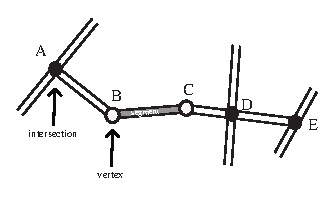
\epsfig{file=compositionOfRoad.eps, height=100px, width=220px}
\caption{The composition of the road network}
\label{fig:composition}
\end{figure}
	
As location data capture by GPS device exposes to distance errors (its standard deviation is around 3 metters at best), map matching is a difficult task. GPSInsights solves this task by enriching the OSM data with a lot of intermediate nodes (beside the nodes declared in OSM) to every road. Thus, each particular location point will be assigned to the road that the closest point belong to. To find closest point, we use KD-tree~\cite{moh2013approximate}. 

	
\begin{figure}[h]
\centering

\epsfig{file=addPointsTofRoad.eps, height=100px, width=220px}
\caption{Add intermedate nodes in road segments}
\label{fig:addPointsToRoad}
\end{figure}
	
Technically, adding intermediate nodes (illustrated in Fig.~\ref{fig:addPointsToRoad}) is done as following. Let's suppose we add a point B into a segment AC in order that the distance between this point and A is $d_{AB}$ ($d_{AB}$ < $d_{AC}$). The coordinate of the point B is determined as following formula:
\[ latitude_{B} = latitude_{A} + (latitude_{C} - latitude_{A}) \ast \frac{d_{AB}}{d_{AC}}\]
\[ longitude_{B} = longitude_{A} + (longitude_{C} - longitude_{A}) \ast \frac{d_{AB}}{d_{AC}}\]
where $d_{AC}$ is the metric distance between the point A and the point C, calculated on $Haversine$ formula~\cite{haversineweb}.

While adding new points, we also remove all intersections and finally build a KD-Tree based on those nodes. Note that a node in the Kd-Tree consists of a coordinate and information of a link which associates it. Therefore, by taking a GPS point into the Kd-Tree and using the vertex-based map matching, we can determine nearest nodes as well as a link it is matched to.
	
\subsection{Detail algorithm}
		
After getting input data from the distributed publish-subscribe messaging service (Apache Kafka), the kd-tree is built and then be broadcasted to all the computing nodes (servers) of the streaming processing engine (Storm or Apache spark). By doing this, in the case that our system uses Spark Streaming, we can keep a read-only variable cached on each machine instead of shipping a copy of it with every tasks, this will help improving the system's performance.
	
As we have a parallelized collection formed, our algorithm will be divided into two phase: a data mapping phase and a data collecting phase. 

\subsubsection{Data Mapping Phase} 
This phase is responsible for matching coordinate of every transportation record q into a concrete segment of the road. In this algorithm, the algorighm consideres the following attributes of q: the latitude, the longitude and the speed. These records will be evaluated by kd-tree cached on each machine to find out which road the recode q belong to. Because of the fact that coordination GPS sent from satellites will have some deviations in comparison with the real coordinate, we have to choose a threshold distance in order to determine whether q belong to the road or not. If the distance is smaller than the threshold distance, it will be much easier for us to conclude that q belongs to the road segment and vice versa. As a result, our algorithm can ignore q that its distance within the road segment is too far from. Therefore, we can enhance the accuracy of our algorithm to some extent.

\subsubsection{Data Collecting Phase} \label{datacollectingphase} In data mapping phase, the transportation data on each time step are transferred to the distributed stream processing engine will be matched into road segments in-parallel. Our algorithm then collectes the output form all the computing nodes to achieve the final statistic results.  In this phase, all the transportation data belong to the same road ID is aggregated. Hence, we can obtain $<$key, value$>$ pairs with the key being the road segment's ID, the value that contains the number of vehicles moving in that road segment and the sum of their speeds $v_{s}$. Then, we calculate the average speed of every links (a section of a road between two intersections, as we described in section \ref{ssec:links}) using the following ``space mean speed'' formula which we will give an detailed explanation in the $appendix$ section.
\[ v_{s} = \frac{N}{\sum_{i=1}^{N}\frac{1}{v_{i}}}\]
where $v_{i}$ is the spot speed of $i^{th}$ vehicle, and n is the number of vehicles.

\section{Experiments}
Our data include about 12,565,521 GPS records collected by vehicles equipped with a GPS receiver from 22/03/2014 to 22/04/2014 in Ho Chi Minh city. Every record consists of speed, GPS coordinate and state of the vehicle and the period of time between two records is 15 minutes. The following table shows the format of the data.

GPSInsights system is set up on a cluster of HPCC super computer, consisting of 4 nodes, one master node and three slave nodes. Each cluster node is equipped with a  8-cores Intel Xeon 2.6GHz CPU, 32GB memory. With this configuration, we have evaluated the performance of GPSInsights, using the dataset shown in section 4.1 to simulate the stream data. Next, we benchmarked the system using Spark Streaming against one using Apache Storm and compared with the common system using Geomesa for map matching (based on the ability of querying K-nearest neighbor search of this database). For all experiments, the results are reported by averaging three runs. 
	
	% 	 Suppermicro SC815TQ-600WB\\ Intel Xeon E5-2670 Processor (20M Cache, 2.6 GHz, 8 Core)\\	 32 GB DDR3 RAM\\	 2*250 GB HDD\\	 FDR 56Gbps Infiniband\\
	
	\begin{figure}[h]
		\centering
		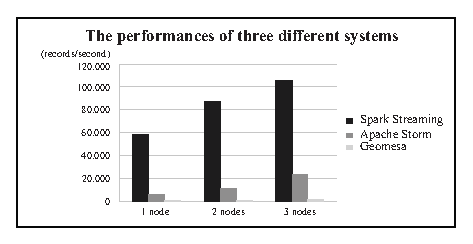
\epsfig{file=thesis-7.eps, height=100px, width=220px}
		\caption{the performances}
		\label{fig:performance}
	\end{figure}

Figure~\ref{fig:performance} presents the performance of GPSInsights using Spark Streaming, one using Apache Storm and the Geomesa system for handling the transport records with the number of slave nodes from 1 to 3. In this experiment, the processing time of the system is measured from the time the streaming processing engine (Spark Streaming or Apache Storm)/Geomesa receives the data from Kafka, until the analytic data  are sent successful to the storage components. It is clear that the number of slave nodes was increased, the execution time of the system reduced steadily. However, with about 52.000 handled records/second (1 node), 86.000 (2 nodes) and more 105.000 (3 nodes), our system using Spark Streaming saw the highest performance, being around 9 times faster than using Apache Storm, while the least one is the Geomesa system, just dealing with around 5000 records per second with 3 slave nodes. The Spark Streaming system achieving the best performance is mainly due to taking the advantage of the in-memory batch handling strategy, we can execute the nearest neighbor search directly in memory by using the map-matching algorithm shown in section 4.

	\begin{figure}[h]
		\centering
		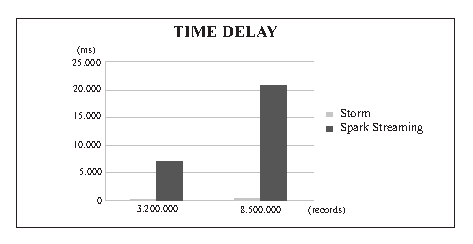
\epsfig{file=thesis-6.eps, height=100px, width=220px}
		\caption{Time delay}
		\label{fig:timedelay}
	\end{figure}
	
Figure~\ref{fig:timedelay} show the time delay of two systems using two different frameworks as the streaming data processing engine for performing the map-matching algorithm in 3.200.000 and 8.500.000 records of the input data. Although the system using Spark Streaming is so much faster than using Storm, one using Storm can it in term of the time delay. Because Storm processes incoming events one at a time , so that its processing latency could be sub-second. Otherwise, after collecting the input data into a batch, Spark Streaming then divide it up into partitions and sent them to slave nodes. So the processing latency of Spark Streaming depends on the batch interval (if the batch interval is 5 seconds, it means that Spark has to wait 5 seconds before starting processing the first batch)  and the number of records packed in the batch (the time for sending partitions to slave nodes is directly proportional to the quantity of records).


\section{Related work}

PostGIS~\cite{posgis} is a spatial database extender for PostgreeSQL object-relational database, adds support for geographic objects allowing location queries to run in SQL. Remember that the relational database has the ability to use information from multiple indexes to determine how best to search for the records that satisfy all query criteria, so it is good for multi-dimension data rather than a key-value store. It is undeniable that PostGis completely meets most of the spatial-temporal query and there are a large number of software products that can use PostGIS as a database backend~\cite{backendposgis}. However, spatio-temporal data sets have seen a rapid expansion in volume and velocity due to the rapid increase of means of transport and GPS device, which is about hundred millions and more records per day. With the reason that the capacity of a PostGIS is only about five hundred millions rows, we have to buy more hardware to meet the demand. However, we will have to cope with many issues such as data management, hardware cost and performance. It is clearly that Accumulo and Geomesa are good for tackle big transport data set.

There are a number of studies on matching GPS observations on a digital map. We can generally classify them into two categories~\cite{yang2005map} Map-matching algorithms using only geometric relationships between GPS data and a digital map and Map-matching consider not only geometric relationships but also the topology of the road network and history of GPS data.
		
		\setlength{\parindent}{0.7cm} Map-matching in first category can be classified by Noh and Kim(1998)~\cite{noh1998map} into the map matching algorithm using the distance of point-to-curve. One using the distance of curve-to-curve and one using the angle of curve-to-curve.
		
		\setlength{\parindent}{0.7cm} Map-matching using the network topology and the data history match the present point to a link based on the result of matching the previous point. However, when the distance between them is higher than a threshold then this method will use only the geometric relationships to match the GPS points to the nearest link.
		
		\setlength{\parindent}{0.7cm} Map-matching using the network topology and the data history are not appropriate for our GPS data which is described in the section~4. Neither of those two categories has demonstration with a scalable algorithm building with the distributed processing engine. 
			
\section{Conclusion and Future Work}
This paper presents GPSInsights, a scalable, extensible and reliable system for continuously processing the massive amounts of vehicle data. We described the main components of the system, explain why to go for them, and the map-matching algorithm being inside of. We also described the method to improve the system, insuring the vehicle data which are handled exactly one, by rewriting the Spark Streaming's receiver and building the simple NoSQL transaction for MongoDb. In addition, through conducting the vehicle data statistic, we proved the GPSInsights' potential to address an increasing number of the problem classes relating massive GPS vehicle data.

In the future work, we intent to pursue the system in three directions. Firstly, We will use the advance map-matching algorithm with higher accurate on low-sampling-rate vehicle data, about 15 seconds or less. Secondly, GPSInsights will be installed new algorithm for predicting future traffic conditions based on real-time data.Finally, the system will be improved to find the fastest path depending on the travel times of each road segment.
%
% The following two commands are all you need in the
% initial runs of your .tex file to
% produce the bibliography for the citations in your paper.
\bibliographystyle{abbrv}
\bibliography{dasfaa2015}  % sigproc.bib is the name of the Bibliography in this case
% You must have a proper ".bib" file
%  and remember to run:
% latex bibtex latex latex
% to resolve all references
%
% ACM needs 'a single self-contained file'!
%
%APPENDICES are optional
%\balancecolumns
\appendix \label{appendix}

\section{Space mean speed}
The formula in $Data Collecting Phase$ (\ref{datacollectingphase}) section could be determined as follow:

Let $t_{i}$ is the time the vehicle having a speed $v_{i}$ take to complete a link having a length D. So
	\[ t_{i} = \frac{1}{v_{i}} \] 

And the average speed $v_{s}$ of all vehicles traveling in the link is their total distance divided by their total time.
	\[v_{s} = \frac{\sum_{i=1}^{N} D}{\sum_{i=1}^{N} t_{i}}\]
It's equal to:
	\[v_{s} = \frac{N \ast D}{\sum_{i=1}^{N} \frac{D}{v_{i}}} = \frac{N}{\sum_{i=1}^{N}\frac{1}{v_{i}}} \]

\section{the visual display system}

We also made the system to show periodically the statistic result for users. This display system is built based on Java Spring MVC framework ~\cite{javaspringmvc} and the Open Street Map data~\cite{openstreetmap}, getting the data from the distributed result queue through the connect module illustrated as the following figure:

\begin{figure}[h]
	\centering
	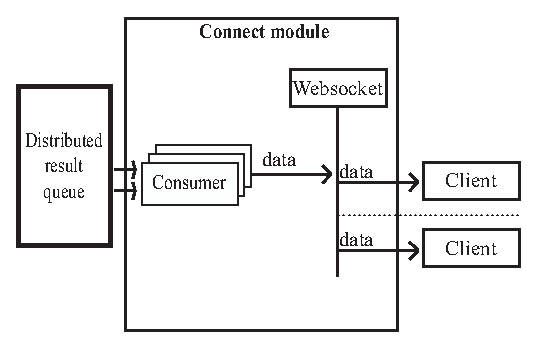
\epsfig{file=connectmodule.eps, height=110px, width=220px}
	\caption{The connect module}
	\label{fig:connectmodule}
\end{figure}

There are two main components in this module: Kafka's consumers and WebSocket~\cite{websocket}. Using WebSocket is in order to send the data to many clients in a short period of time. While the purpose of choosing the consumer is to minimize the waiting time of the data processing engine when pushing the final statistic results to the connect module, by taking advantage of read/write in parallel of Spark Streaming/Apache Storm and especially Apache Kafka. After receiving the data from the connect module, the display system will draw them as follow:

	\begin{figure}[h]
		\centering
		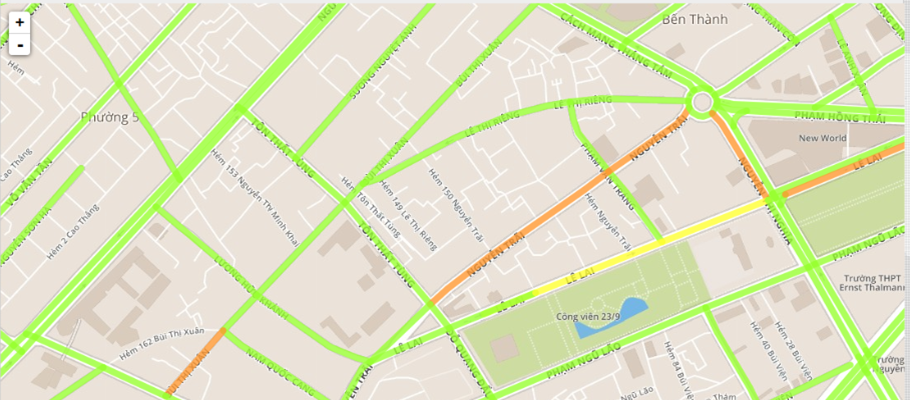
\includegraphics[height=110px,width=220px]{Picture1}
		\caption{Showing the statistic results for users}
	\end{figure}

Where the green line expresses the road having the average speed 30 km/h and over, the yellow one shows the average speed from 15 km/h to 30 km/h, the orange one for 5-15 km/h and the red line means having the traffic jam in the road. Also, the system will update automatically as soon as receiving the new results.

\section{the pseudocode of algorithm} 
\medskip
\noindent
The below pseudocode illustrates the algorithm installed in our system using Spark Streaming, for instance.

\begin{verbatim}
		
		// kdTree: a KD-Tree build up from nodes of OSM data
		// input: a list containing data queried from accumulo
		// output: a list of tuple2<key, value> with key being a roadID 
		// and value being a number of vehicle and average speed
		// scc: a Java Spark Context variable
		// lines: distributed datasets
		// broadcastVal: keep a read-only variable of the kdTree
		// currentPoint: GPS vehicle 
		// nearestNode: nearest node of current point
		// distance: distance between currentPoint and nearestNode
		// listRoad: a <key,value> generated after maping lines with key
		// being a roadID, value being a iterable of vehicleID and speed
		// result: a <key, value> generated after maping listRoad with key 
		// being a roadID, value being vehicle volume and average speed
		Build up the kdTree
		Broadcast<KDTree<GeoName>> broadcastVal = scc.broadcast(kdTree);
		JavaRDD<String> lines = scc.parallelize(input).cache();
		JavaPairRDD<String, Iterable<String>> listRoad = lines
		    .mapToPair(New PairFunction<String, String, String>() {
		        Public Tuple2<String, String> call(String p1) 
		            Throws Exception {
		            nearestNode = broadcastVal.value().
		                              findNearest(currentPoint);	
		            If distance > threshold then
		                roadID = Null;
		            Else 
		                roadID = nearestNode.toString();
		                vehicleID = currentPoint.ID;
		                speed = currentPoint.speed;
		                attributes = vehicleID + speed;
		            end If;
		        Return New Tuple2<String, String>(roadID, attributes);
		    }).groupByKey().cache();
		JavaPairRDD<String, String> result = listRoad
		    .mapToPair(New PairFunction<Tuple2<String, Iterable<String>>, 
		               String, String>() {
		        Public Tuple2<String, String> call(Tuple2<String,
		               Iterable<String>> tuple1) Throws Exception {
		            numberOfVehicle = Count the number of element
		                              in iterable value of listRoad;
		            averageSpeed = Calculate average speed from
		                              iterable value of listRoad;
		            statistic = numberOfVehicle + averageSpeed;
		        Return New Tuple2<String, String>(roadID, statistic);
		    });
		Collect result
		    output = result.collect();
		end Collect;

\end{verbatim}
%
\noindent

\end{document}























